\chapter{Implementation}
\section{Parser}

The parser was written in TypeScript. Although there are many frameworks that could have been used for lexical and syntactic analysis, these were not chosen. The main reason for this is that the parser was meant to be used within a website. In particular, it was expected that the parser became an node package manager (NPM) package. Moreover, TML is quite a simple language, making this task relatively easy and short.

\begin{figure}[htb]
    \centering
    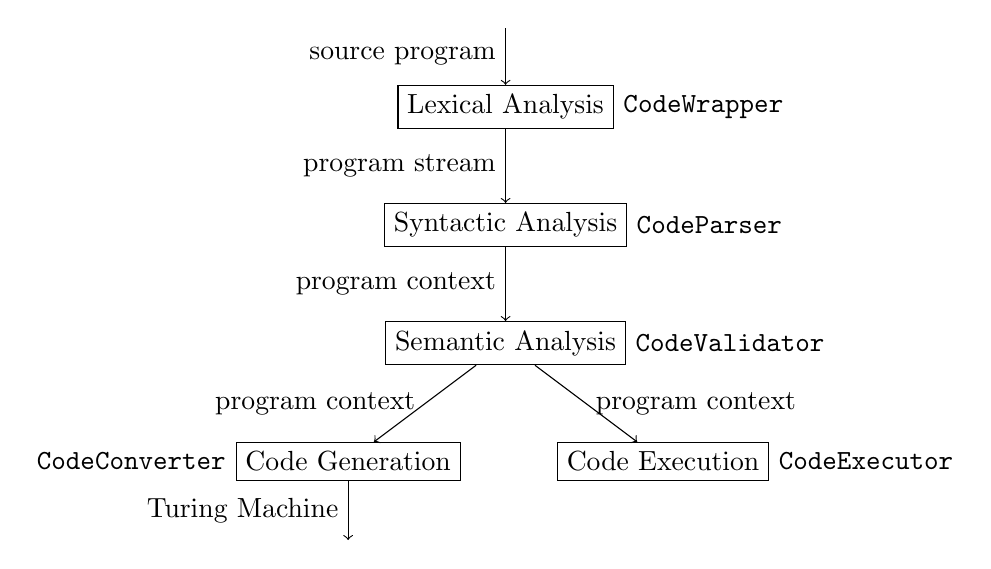
\begin{tikzpicture}
        \node[draw, label={0:\texttt{CodeWrapper}}] (CW) at (0, 0) {Lexical Analysis};
        \node[draw, label={0:\texttt{CodeParser}}] (CP) at (0, -1.5) {Syntactic Analysis};
        \node[draw, label={0:\texttt{CodeValidator}}] (CV) at (0, -3) {Semantic Analysis};
        \node[draw, label={180:\texttt{CodeConverter}}] (CC) at (-2, -4.5) {Code Generation};
        \node[draw, label={0:\texttt{CodeExecutor}}] (CE) at (2, -4.5) {Code Execution};

        \draw[->] (0, 1) -- node[left] {source program} (CW);
        \draw[->] (CW) -- node[left] {program stream} (CP);
        \draw[->] (CP) -- node[left] {program context} (CV);
        \draw[->] (CV) -- node[left] {program context} (CC);
        \draw[->] (CV) -- node[right] {program context} (CE);
        \draw[->] (CC) -- node[left] {Turing Machine} (-2, -5.5);
    \end{tikzpicture}
    \caption{The parsing process. The process is given inside the box. The class used to achieve the process is given in label, outside of the box. The flow of data is also shown.}
    \label{fig:parsing_process}
\end{figure}

The entire parsing process is summarised in Figure \ref{fig:parsing_process}.


\subsection{Lexical Analysis}

During lexical analysis, a stream of source code was produced. Although the source code was not enriched into tokens, the position of the code was tracked. This was to ensure that, in case of an error, the right section of code could be highlighted. This is done using the class \texttt{CodeWrapper}. 

To produce a stream of tokens, the iterator design pattern was used. The iterator design pattern allows us to get the current value from a collection in a way that abstracts the data structure (\cite{gamma1995design}). In particular, the pattern was used to abstract the string representation of the source code and return a single entry from the code at a time. 

\subsection{Syntactic Analysis}
\begin{figure}[htb]
    \centering
    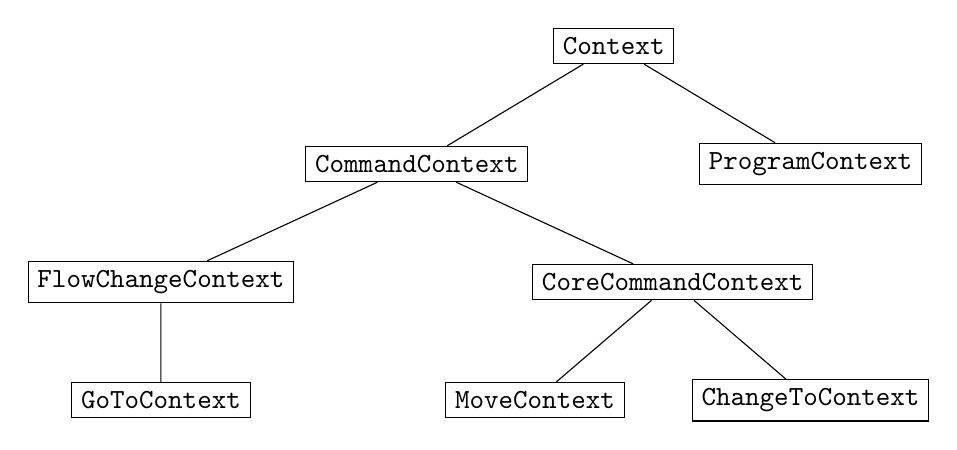
\begin{tikzpicture}[
        level 1/.style={sibling distance=5cm},
        level 2/.style={sibling distance=6.5cm},
        level 3/.style={sibling distance=3.5cm},
    ]
        \node[draw] {\texttt{Context}}
        child {
            node[draw] {\texttt{CommandContext}}
            child {
                node[draw] {\texttt{FlowChangeContext}}
                child {
                    node[draw] {\texttt{GoToContext}}
                }
            }
            child {
                node[draw] {\texttt{CoreCommandContext}}
                child {
                    node[draw] {\texttt{MoveContext}}
                }
                child {
                    node[draw] {\texttt{ChangeToContext}}
                }
            }
        }
        child {
            node[draw] {\texttt{ProgramContext}}
        };
    \end{tikzpicture}
    \caption{A snippet of the \texttt{Context} class hierarchy. All the non-leaf classes are abstract.}
    \label{fig:context_hierarchy}
\end{figure}

Next, the code is parsed. This is done using the class \texttt{CodeParser}. 

The result of the parsing is a \texttt{ProgramContext}, which represents the root of the AST. Subclasses of the \texttt{Context} class are used to represent different statements in the class, such as \texttt{MoveContext} for \textit{move} commands and \texttt{GoToContext} for \textit{goto} commands. A snippet of the class hierarchy for \texttt{Context} is shown in Figure \ref{fig:context_hierarchy}.

The parsing process results in the construction of the AST, such as the one in Figure \ref{fig:TML_AST}. To descend to a child, we make use of the instance fields. For instance, \texttt{ProgramContext} has the following fields:
\begin{itemize}
    \item \texttt{alphabet} for \texttt{AlphabetContext}; and
    \item \texttt{modules} for an array of \texttt{ModuleContext}.
\end{itemize}

The parser is recursive-descent and top-down in nature, as we can see in the \texttt{parseProgram} method below.
\begin{lstlisting}[language=TypeScript]
parseProgram() {
    var alphabet = parseAlphabet();
    
    var modules = [];
    while (code.moveNext()) {
        modules.add(parseModule());
    }
    
    return new ProgramContext(position, alphabet, modules);
}
\end{lstlisting}
Note that the code given above is simplified from the actual implementation.

If the program has syntax errors, then it will not be possible to produce an AST. For instance, the alphabet for the program might not been provided. This is detected by the parser since it makes use of predictive parsing. In particular, the parser looks at the next value and determines if it is legal; otherwise, it throws a \texttt{SyntaxError}.

\subsection{Semantic Analysis}
TODO

% We traverse the AST using the visitor design pattern (\cite{gamma1995design}). Here, every node in the AST is represent by some child class of the \texttt{Context} class, e.g. \texttt{IfContext} for if statements. The \texttt{Context} class has an abstract method \texttt{accept} that allows us to visit different nodes. We can then make use of this when traversing the AST.

% We illustrate the visitor design pattern with an example. So, assume that we have the following class to represent if statements.
% \begin{lstlisting}[language=TypeScript]
% class IfContext extends Context {    
%     accept<T>(validator:CodeVisitor<T>):T? {
%         return validator.visitIf(this);
%     }

%     // ... relevant methods for if context
% }
% \end{lstlisting}
%     In that case, we can define the following method to `visit' an if statement and validate it.
% \begin{lstlisting}[language=TypeScript]
% class TypeValidator implements CodeVisitor<Type> {
%     visit(context:Context):Type? {
%         return context.accept(this);
%     }
    
%     // validate that the condition is of type bool 
%     visitIf(ifContext:IfContext):Type? {
%         var type = visit(ifContext.condition);
%         if (type != Type.BOOL) {
%             throw new TypeError("Expected if condition to be of type bool.");
%         }
        
%         return undefined;
%     }

%     // ... other validator methods
% }
% \end{lstlisting}
% When traversing the AST, we typically want to aggregate the result or share the result with the parent. For this reason, we typically return a specific type of values within each visit method. In the example above, we make use of the class \texttt{Type}, which represents the type of the result, if relevant.

% To run the \texttt{TypeValidator}, we visit the entire program.

% The advantage of using the visitor design pattern is that we can traverse all the nodes without altering any of the \texttt{Context} classes; we can just construct another \texttt{Visitor} class. However, if we wanted to add another \texttt{Context} subclass, then we would need to amend all the \texttt{Visitor} classes. We expect the language to be pretty static, so this is perfectly fine in our case.



\subsection{TM Generation}
TODO

\subsection{Code Execution}
TODO

% TODO: Parser makes use of the visitor design pattern, specify in particular what each one uses
% TODO: Some validation rules are given
% TODO: TM representation is given
% TODO: TM converter and TML converter are explained
% TODO: Describe some non-trivial stuff to write, e.g. breaking from the visitor design pattern to allow for non-useless code

\section{Product}
TODO
% TODO: Website was written in react for its rich set of frameworks
% TODO: The FSM is created using graphviz. Constructs an aesthetically pleasing FSM given the nodes. Uses DOT notation. Initial attempt was to do it myself and create an algorithm that works, but decided instead to do this. This does still have limitations which are discussed in future work
% TODO: The editor comes from monaco framework
% TODO: d3 framework used to show tape transitions (move, change of tape value)
